\begin{figure}
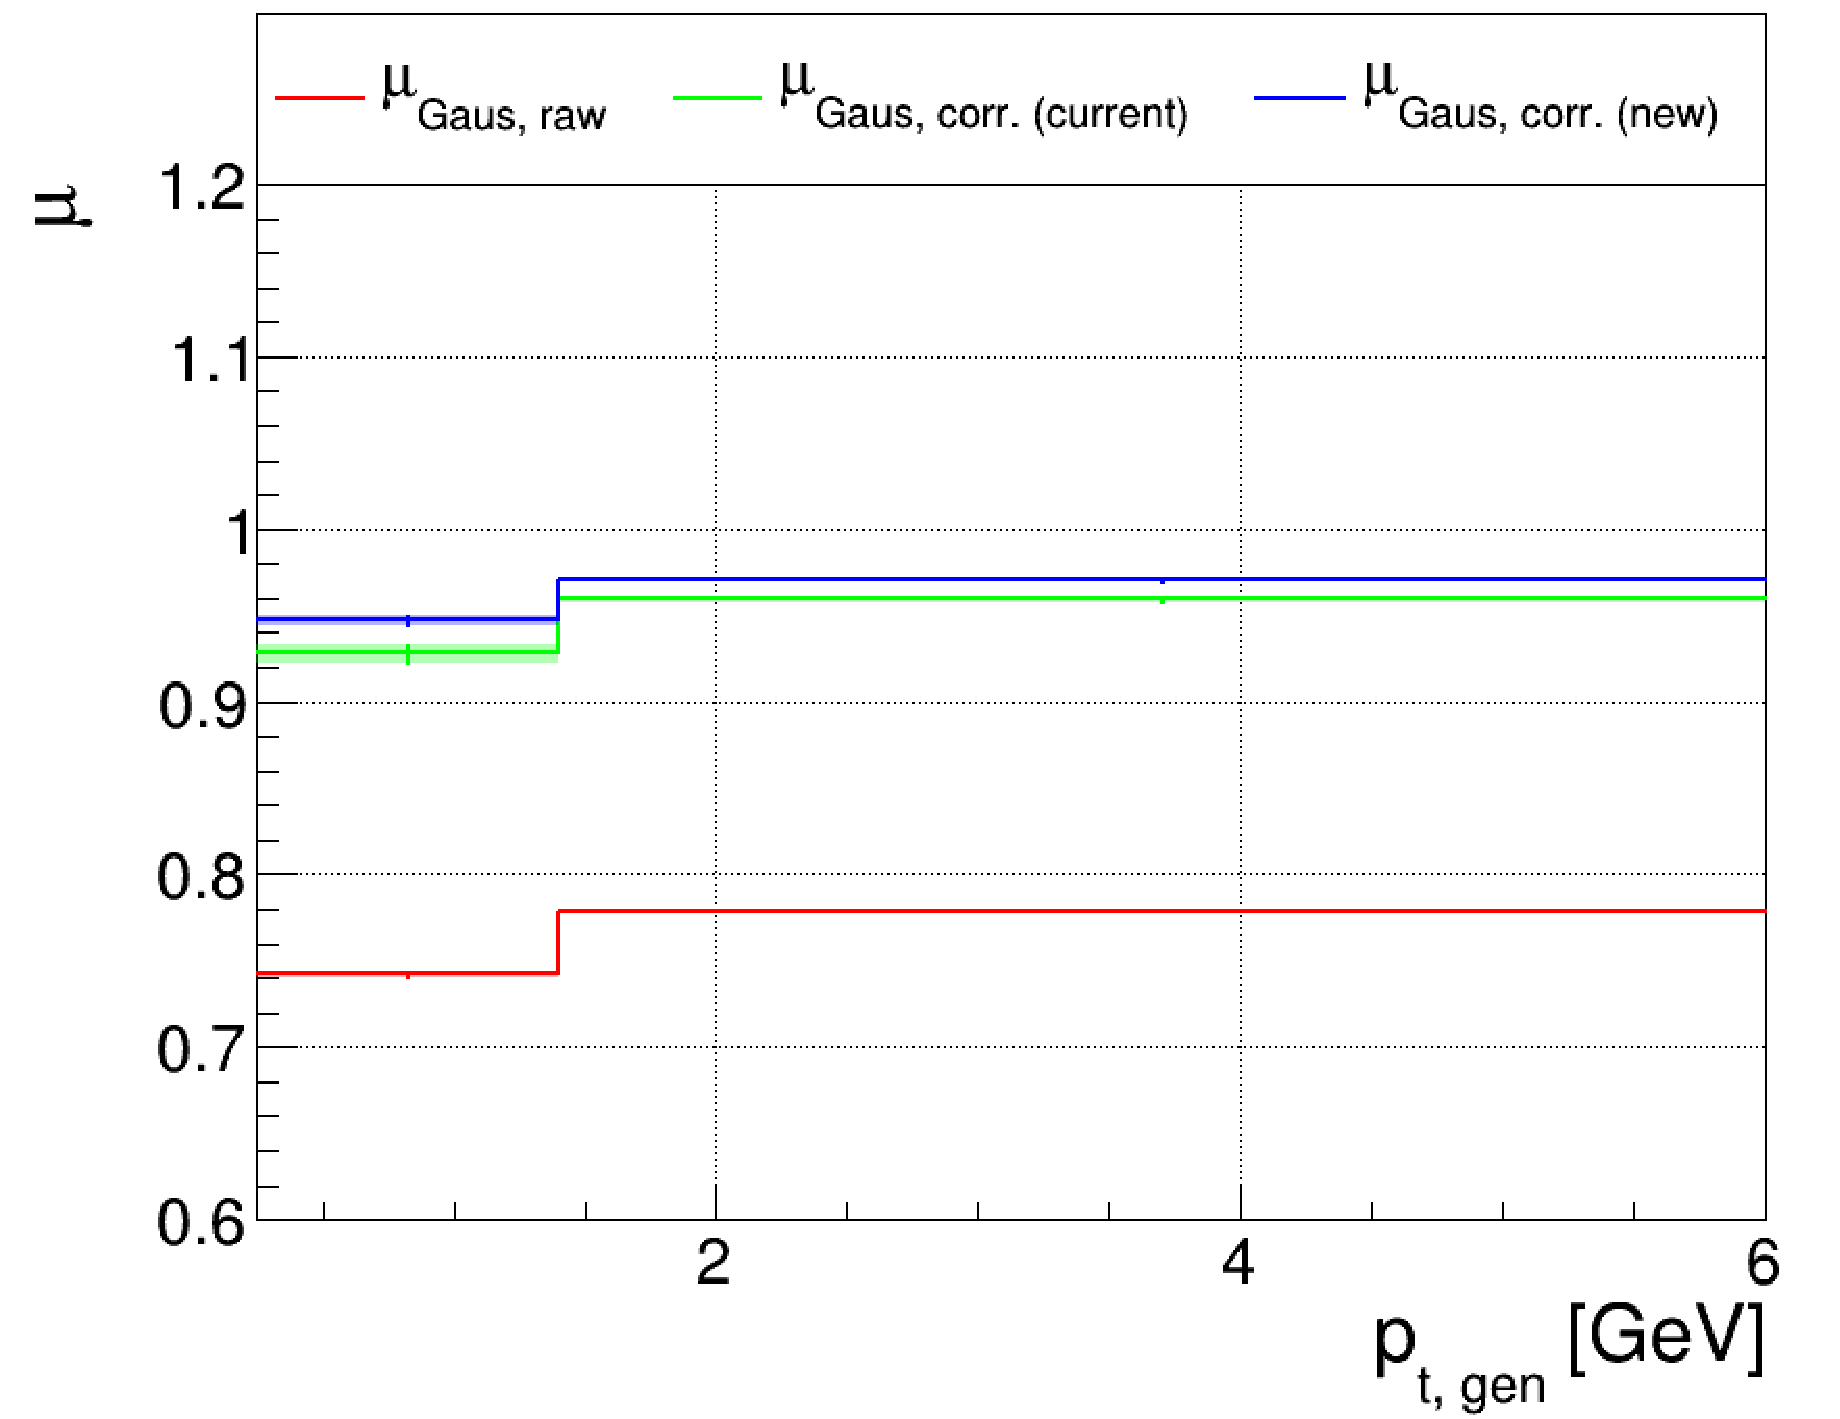
\includegraphics[width=0.495\textwidth]{./plots_pdf/ECAL_plots/plotsNOPU/EB/ZS/pdf/GENPT/EBZS_GENPT_0000_0006_MuOverBins.pdf}
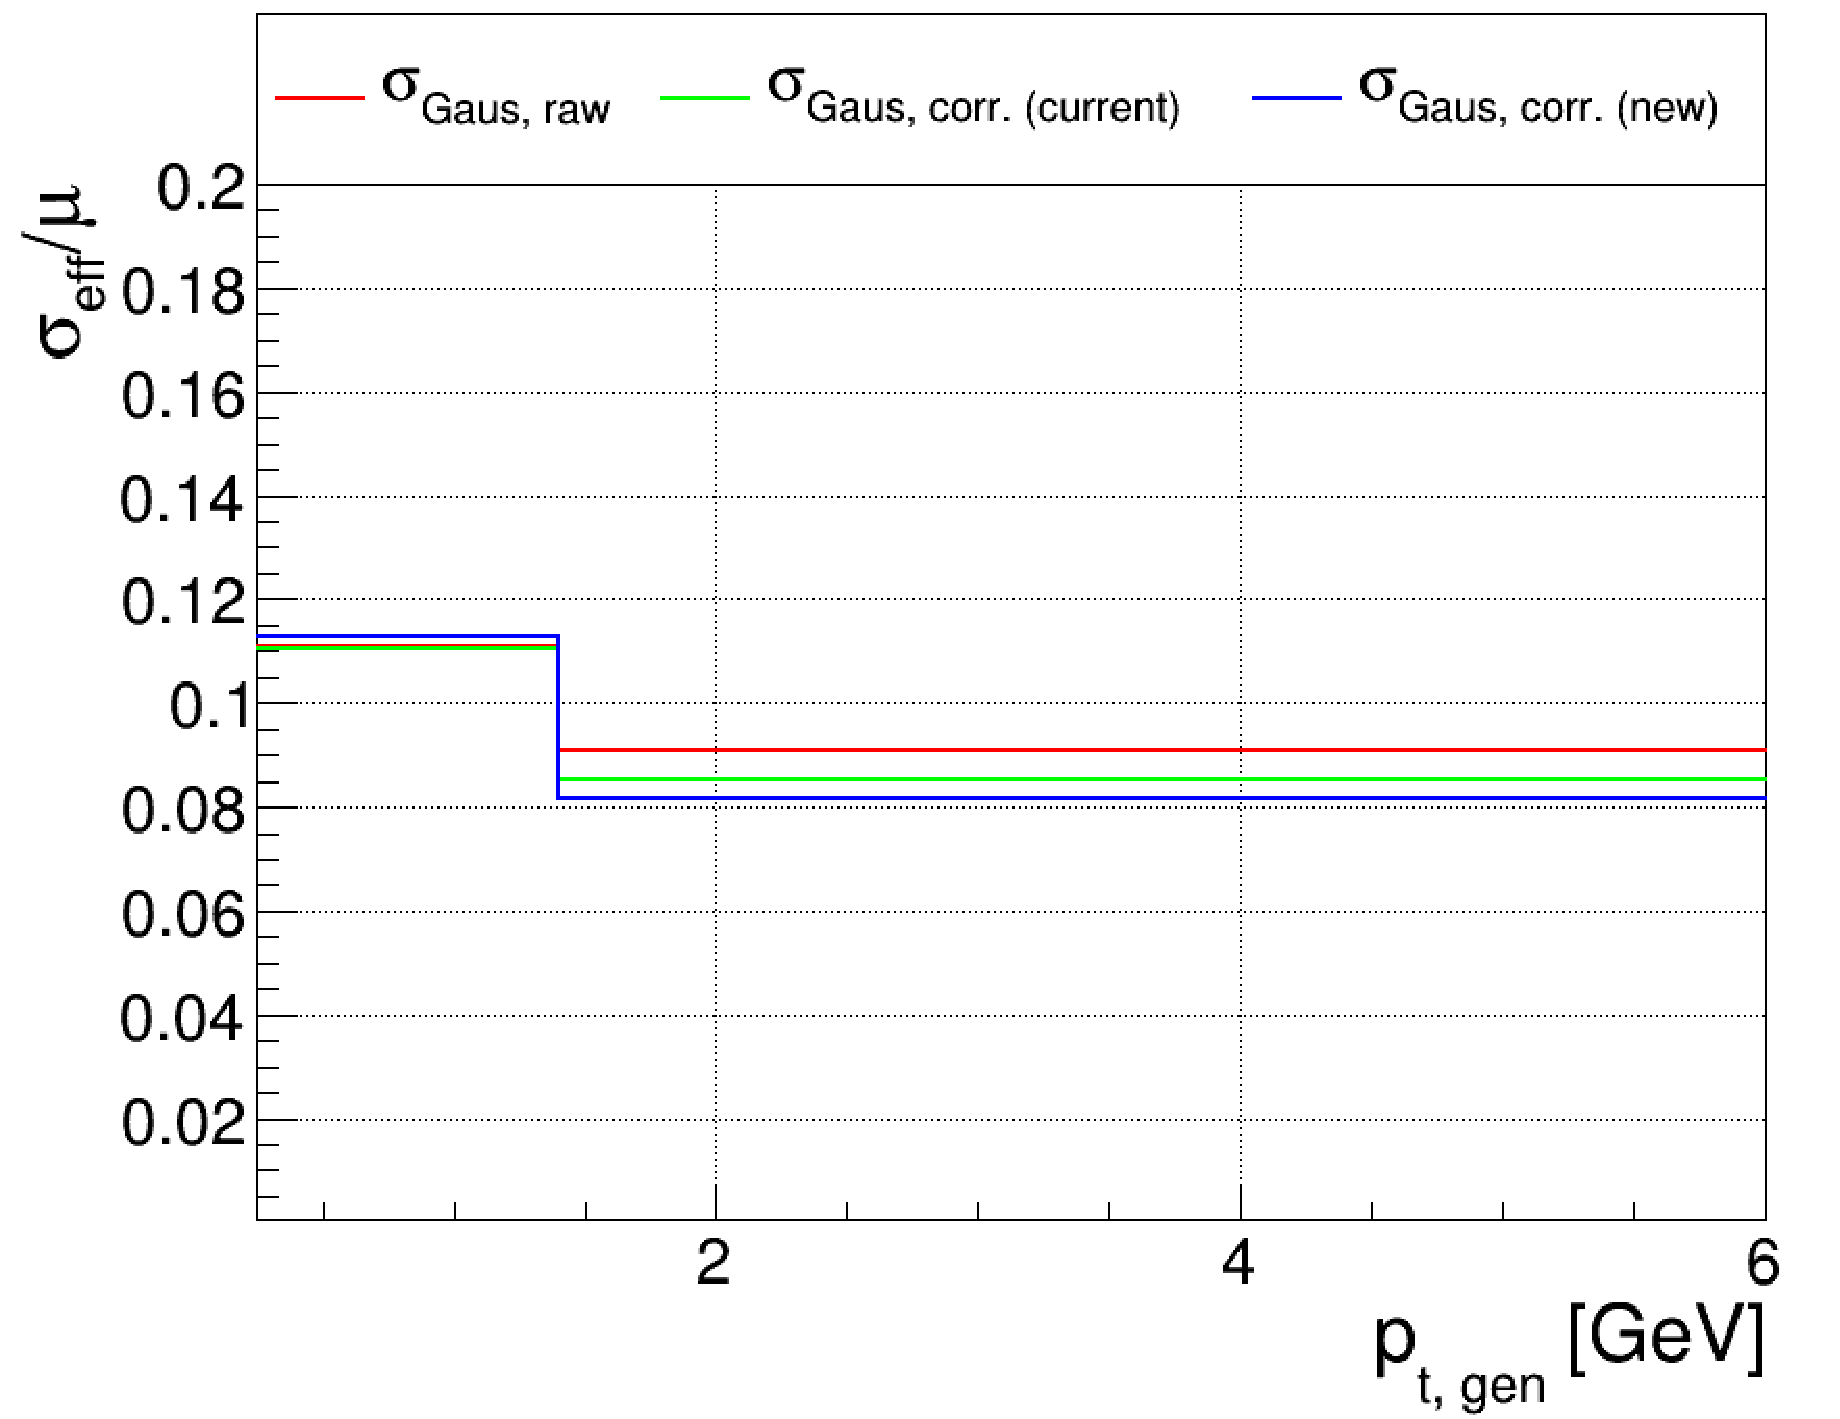
\includegraphics[width=0.495\textwidth]{./plots_pdf/ECAL_plots/plotsNOPU/EB/ZS/pdf/GENPT/EBZS_GENPT_0000_0006_EffSigmaOverBins.pdf}

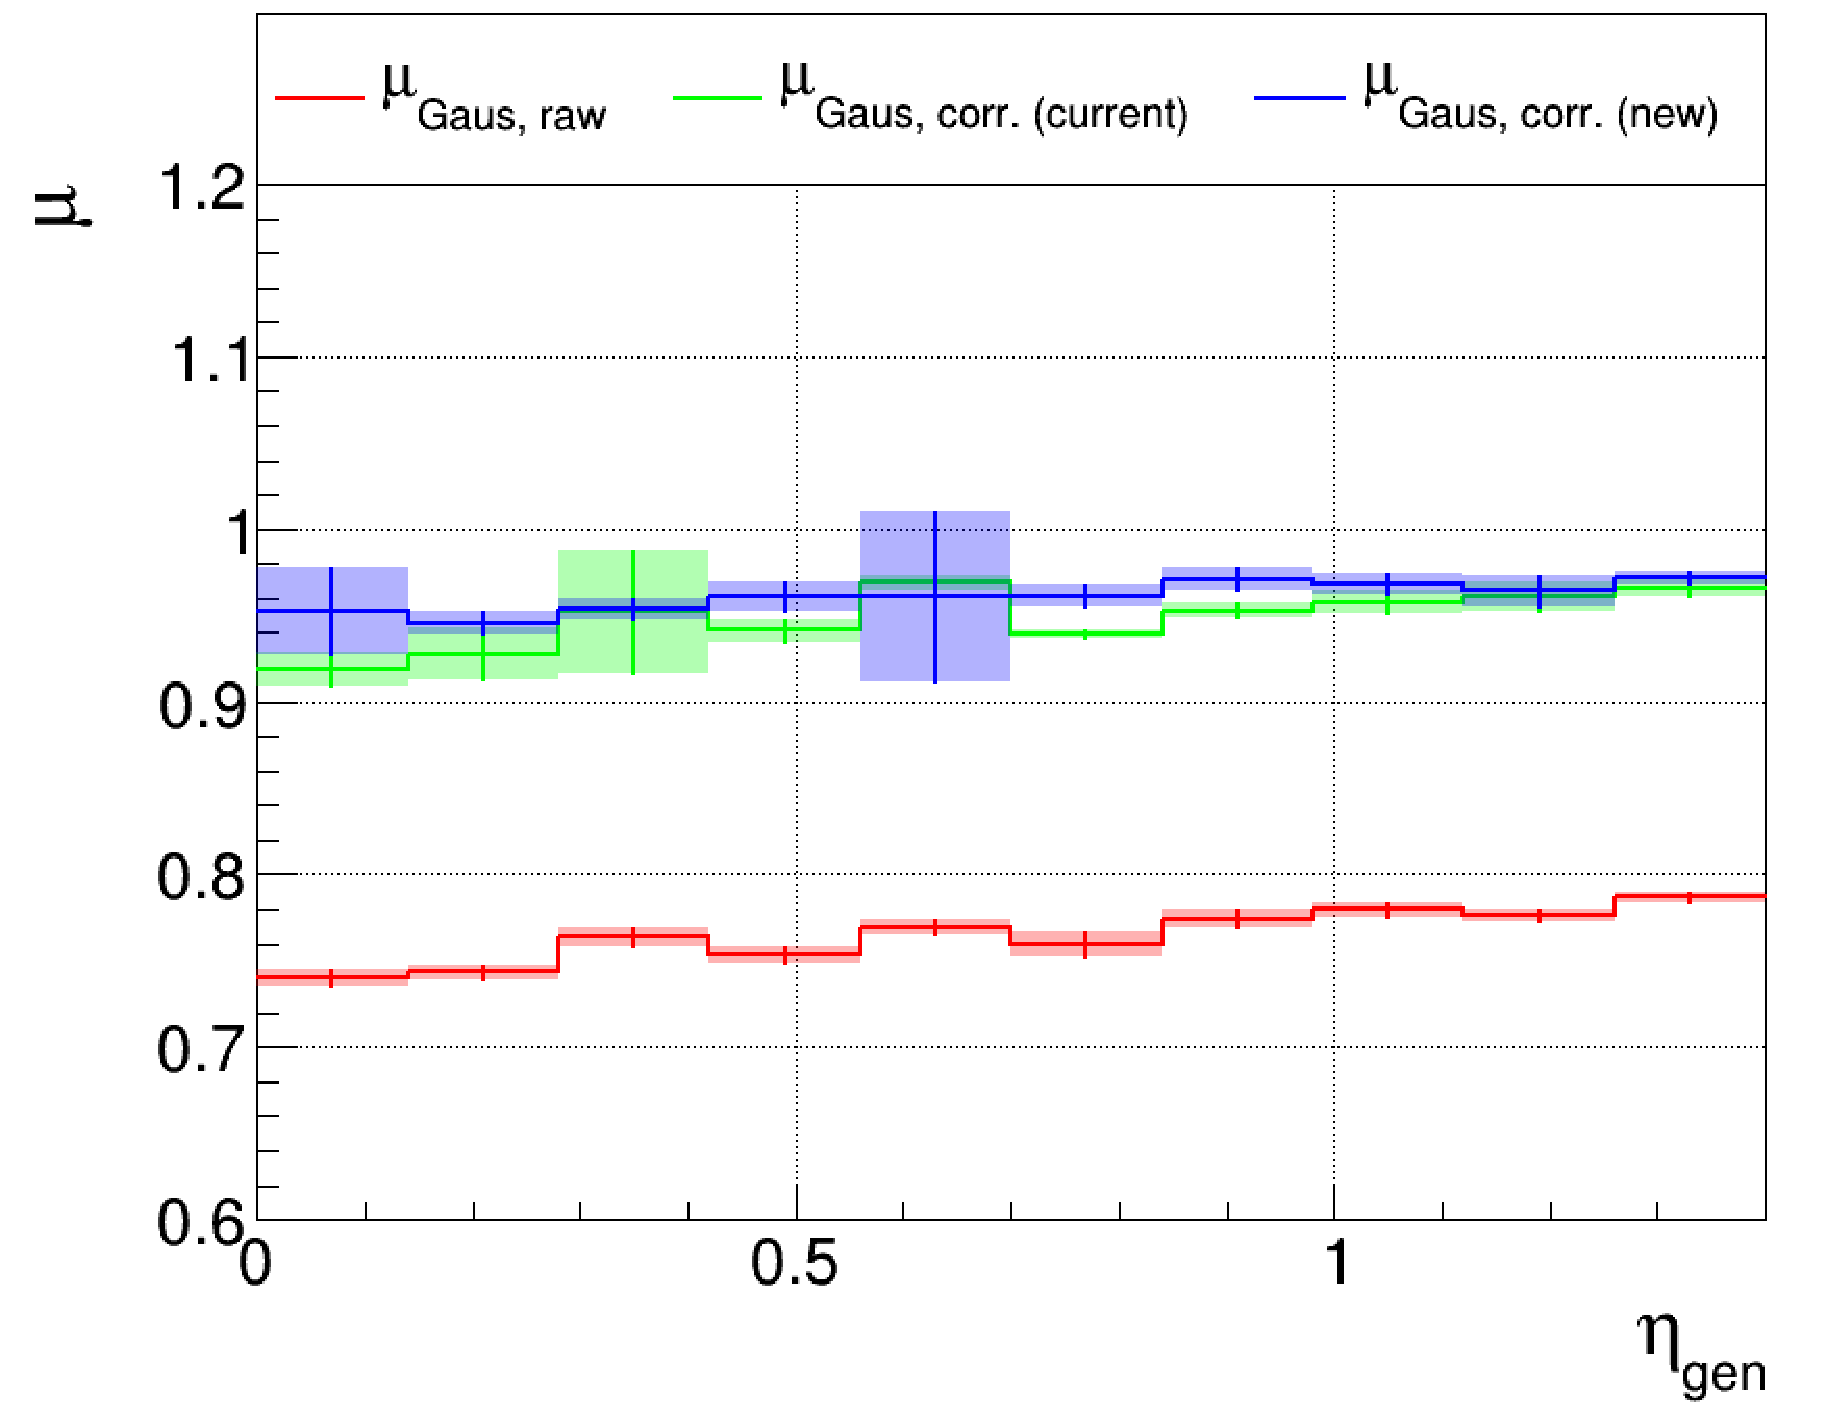
\includegraphics[width=0.495\textwidth]{./plots_pdf/ECAL_plots/plotsNOPU/EB/ZS/pdf/GENETA/EBZS_GENETA_0000_0006_MuOverBins.pdf}
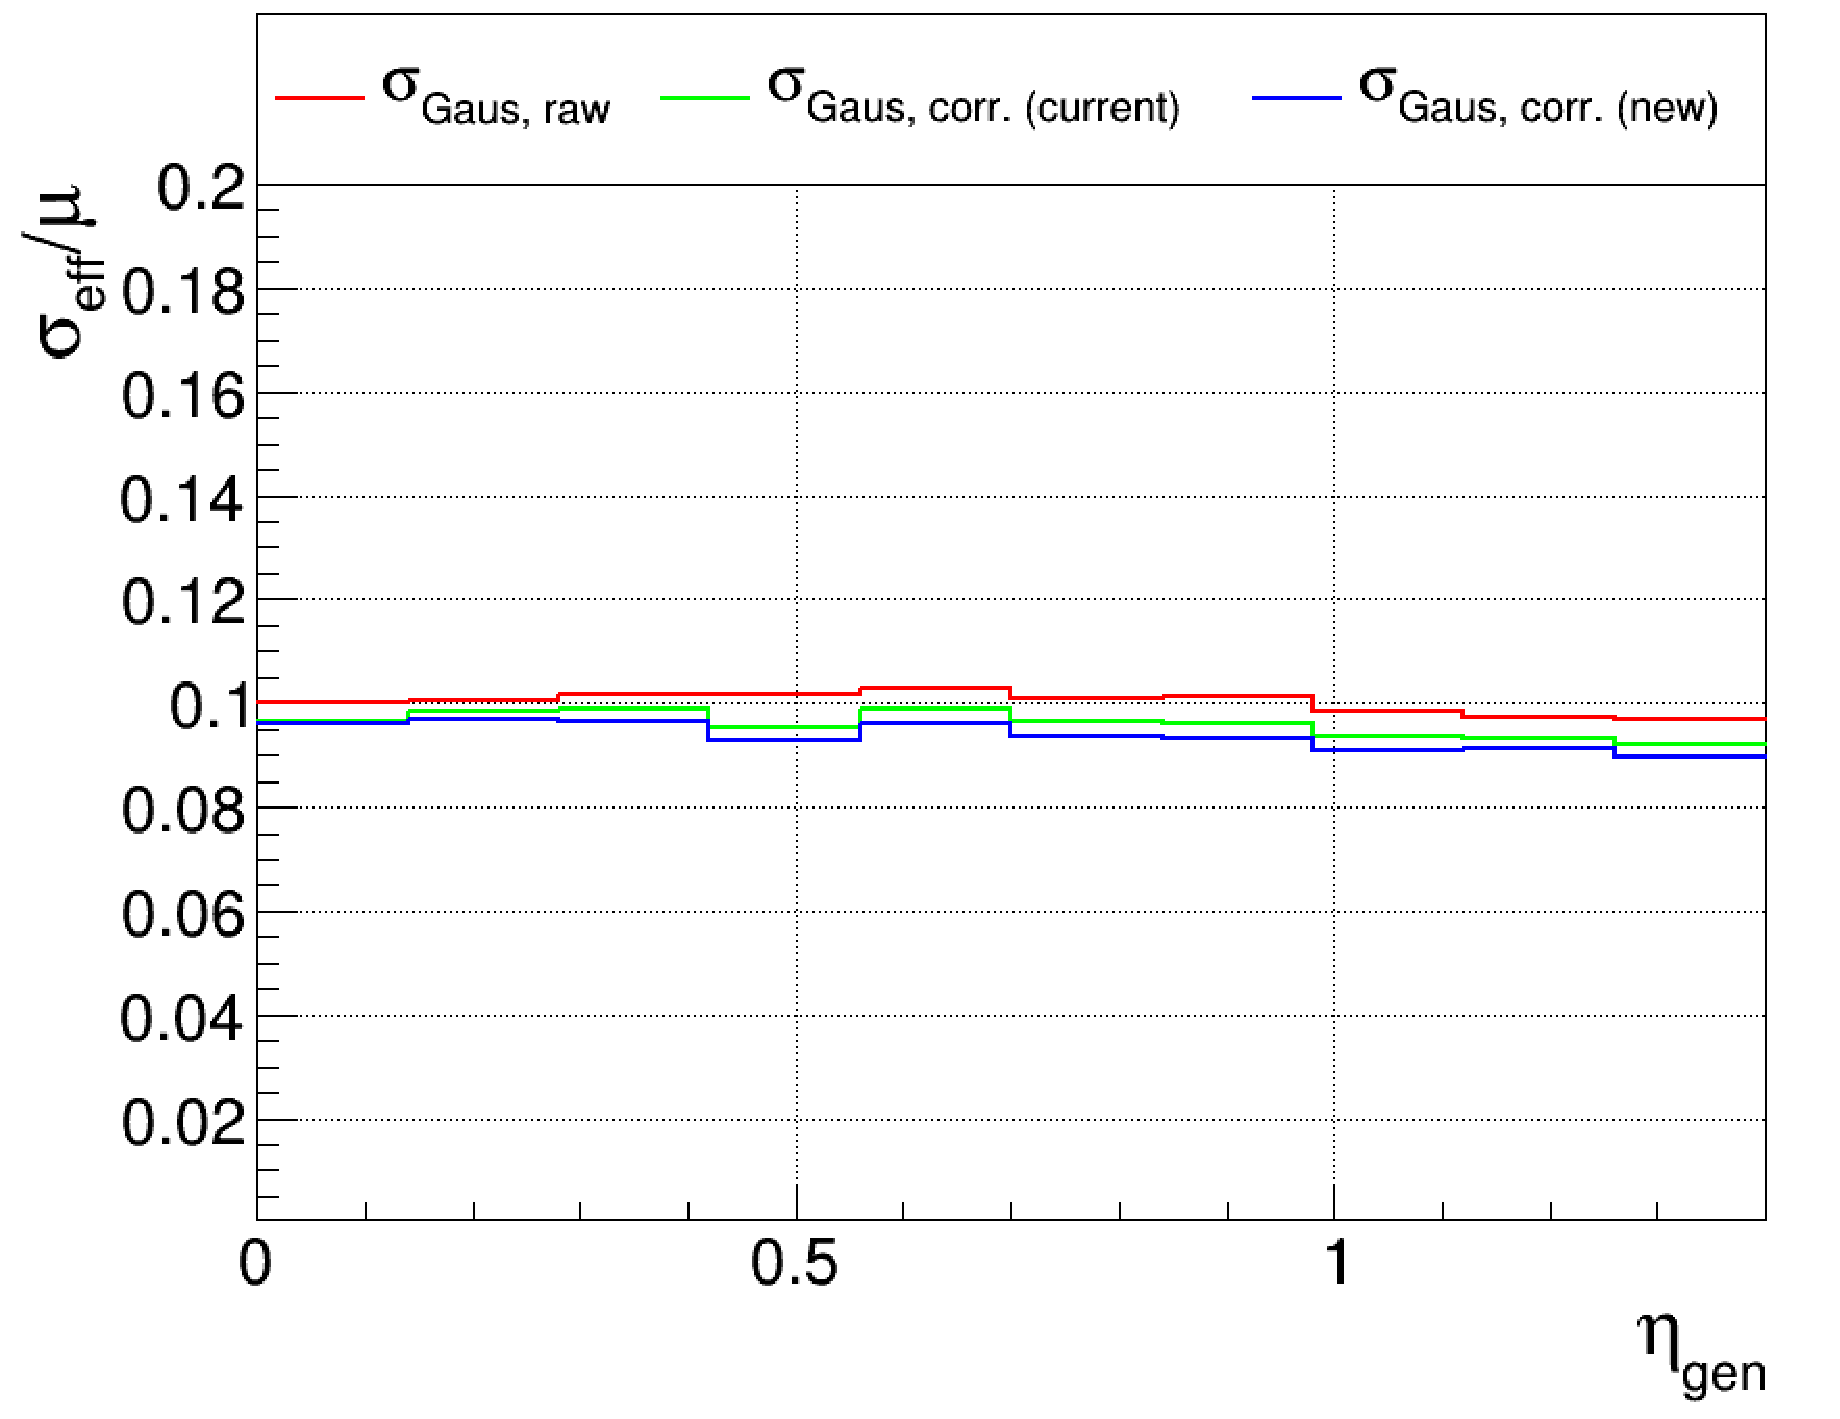
\includegraphics[width=0.495\textwidth]{./plots_pdf/ECAL_plots/plotsNOPU/EB/ZS/pdf/GENETA/EBZS_GENETA_0000_0006_EffSigmaOverBins.pdf}
\caption[$\mu$ ($\sigma_\mathrm{eff}$) vs. \pt of PF ECAL cluster - EB ZS readout NoPU scenario]{Mean response (resolution) defined by raw PF ECAL clusters (red), the calibration derived earlier in Run~3 based on 126X (green), and the new correction from the 2024 simulation sample based on 133X (blue). \pt 0--6\GeV NoPU EB ZS readout NoPU scenario.}
\end{figure}

%% \begin{figure}
%% 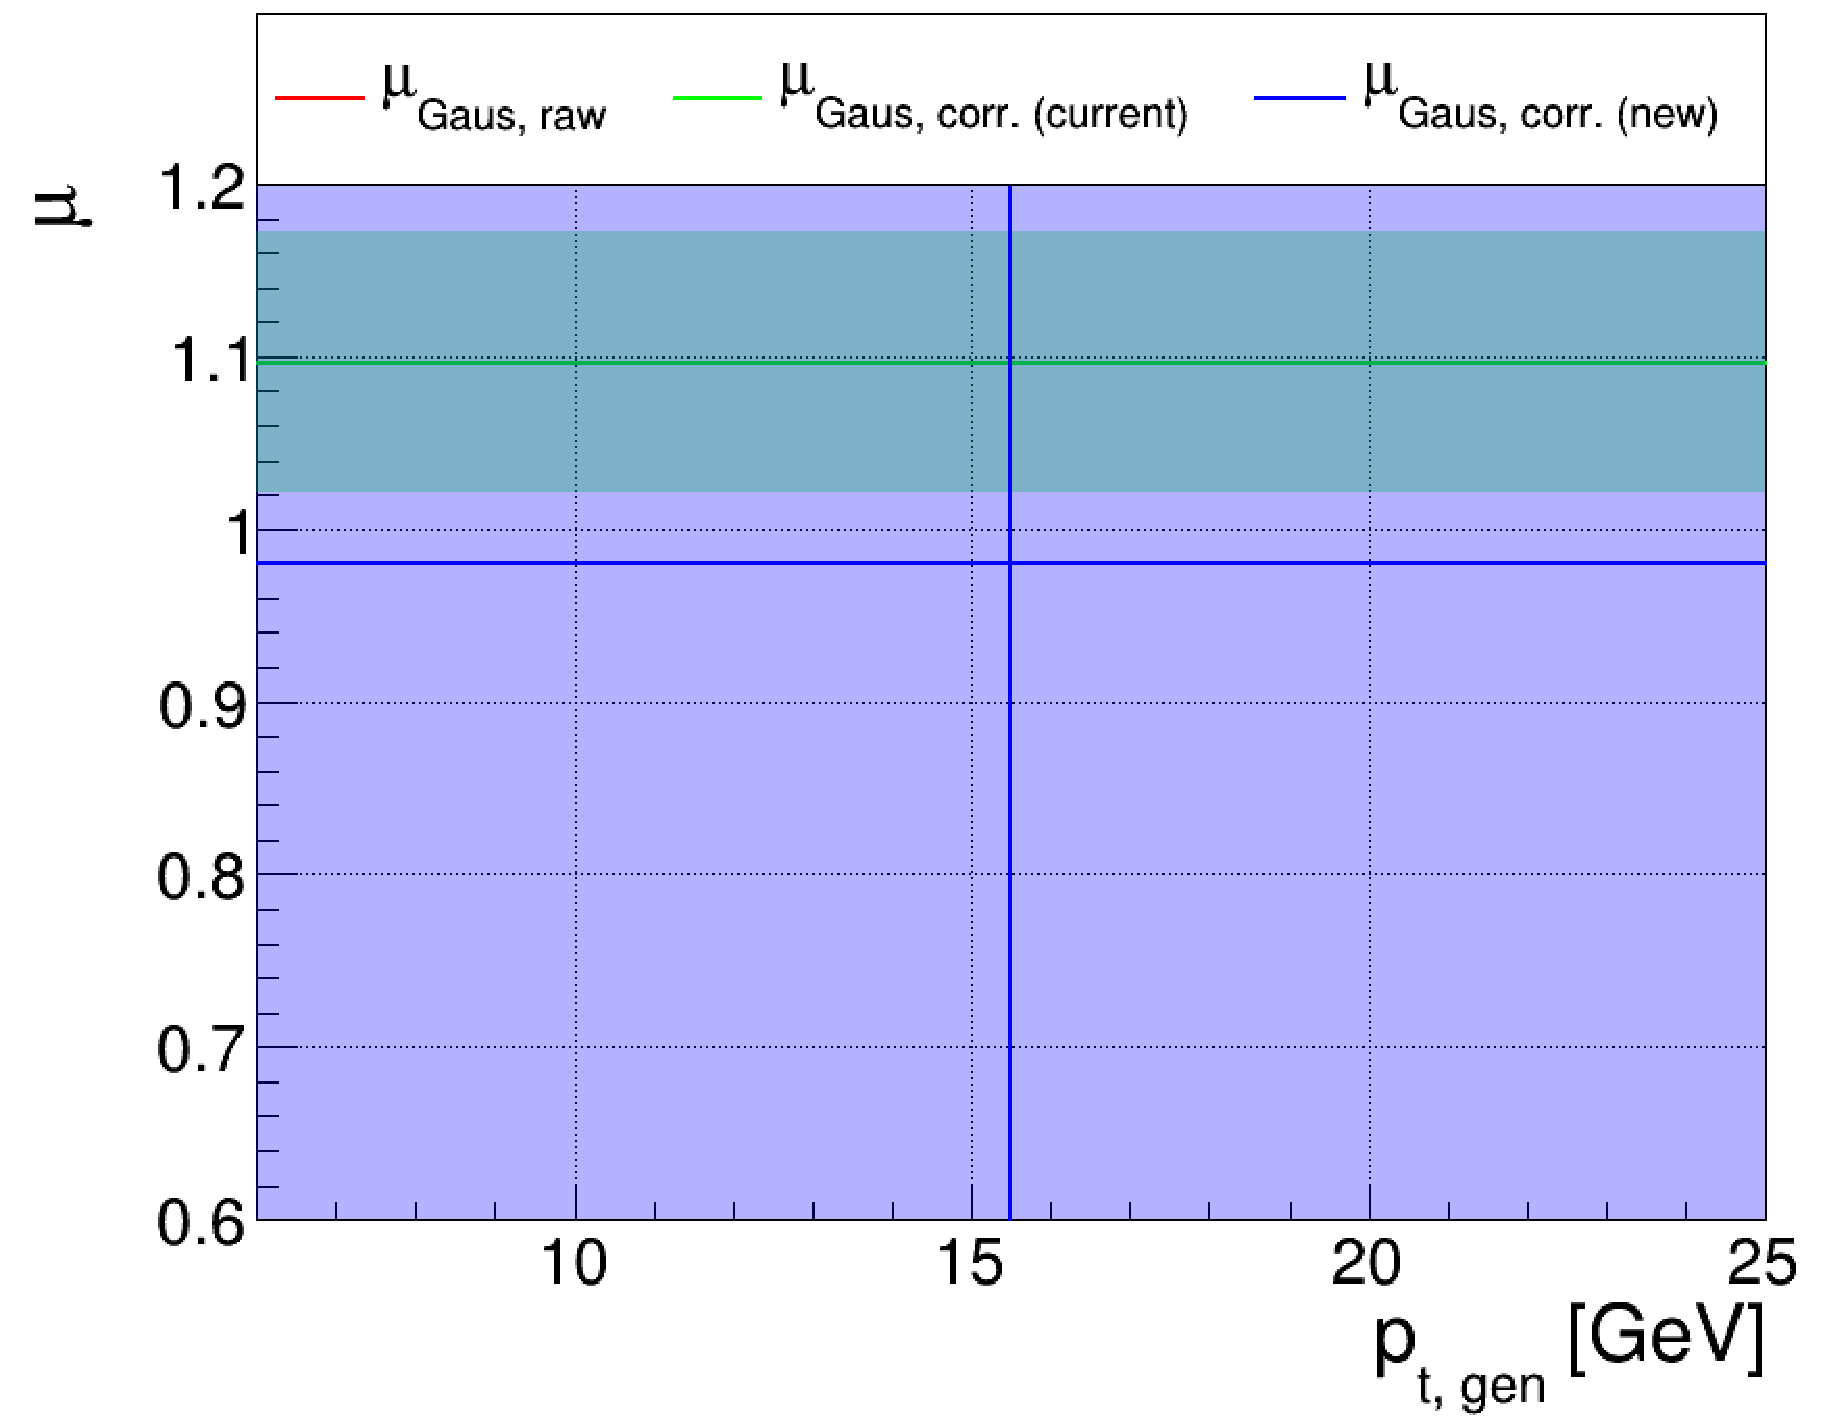
\includegraphics[width=0.495\textwidth]{./plots_pdf/ECAL_plots/plotsNOPU/EB/ZS/pdf/GENPT/EBZS_GENPT_0006_0025_MuOverBins.pdf}
%% 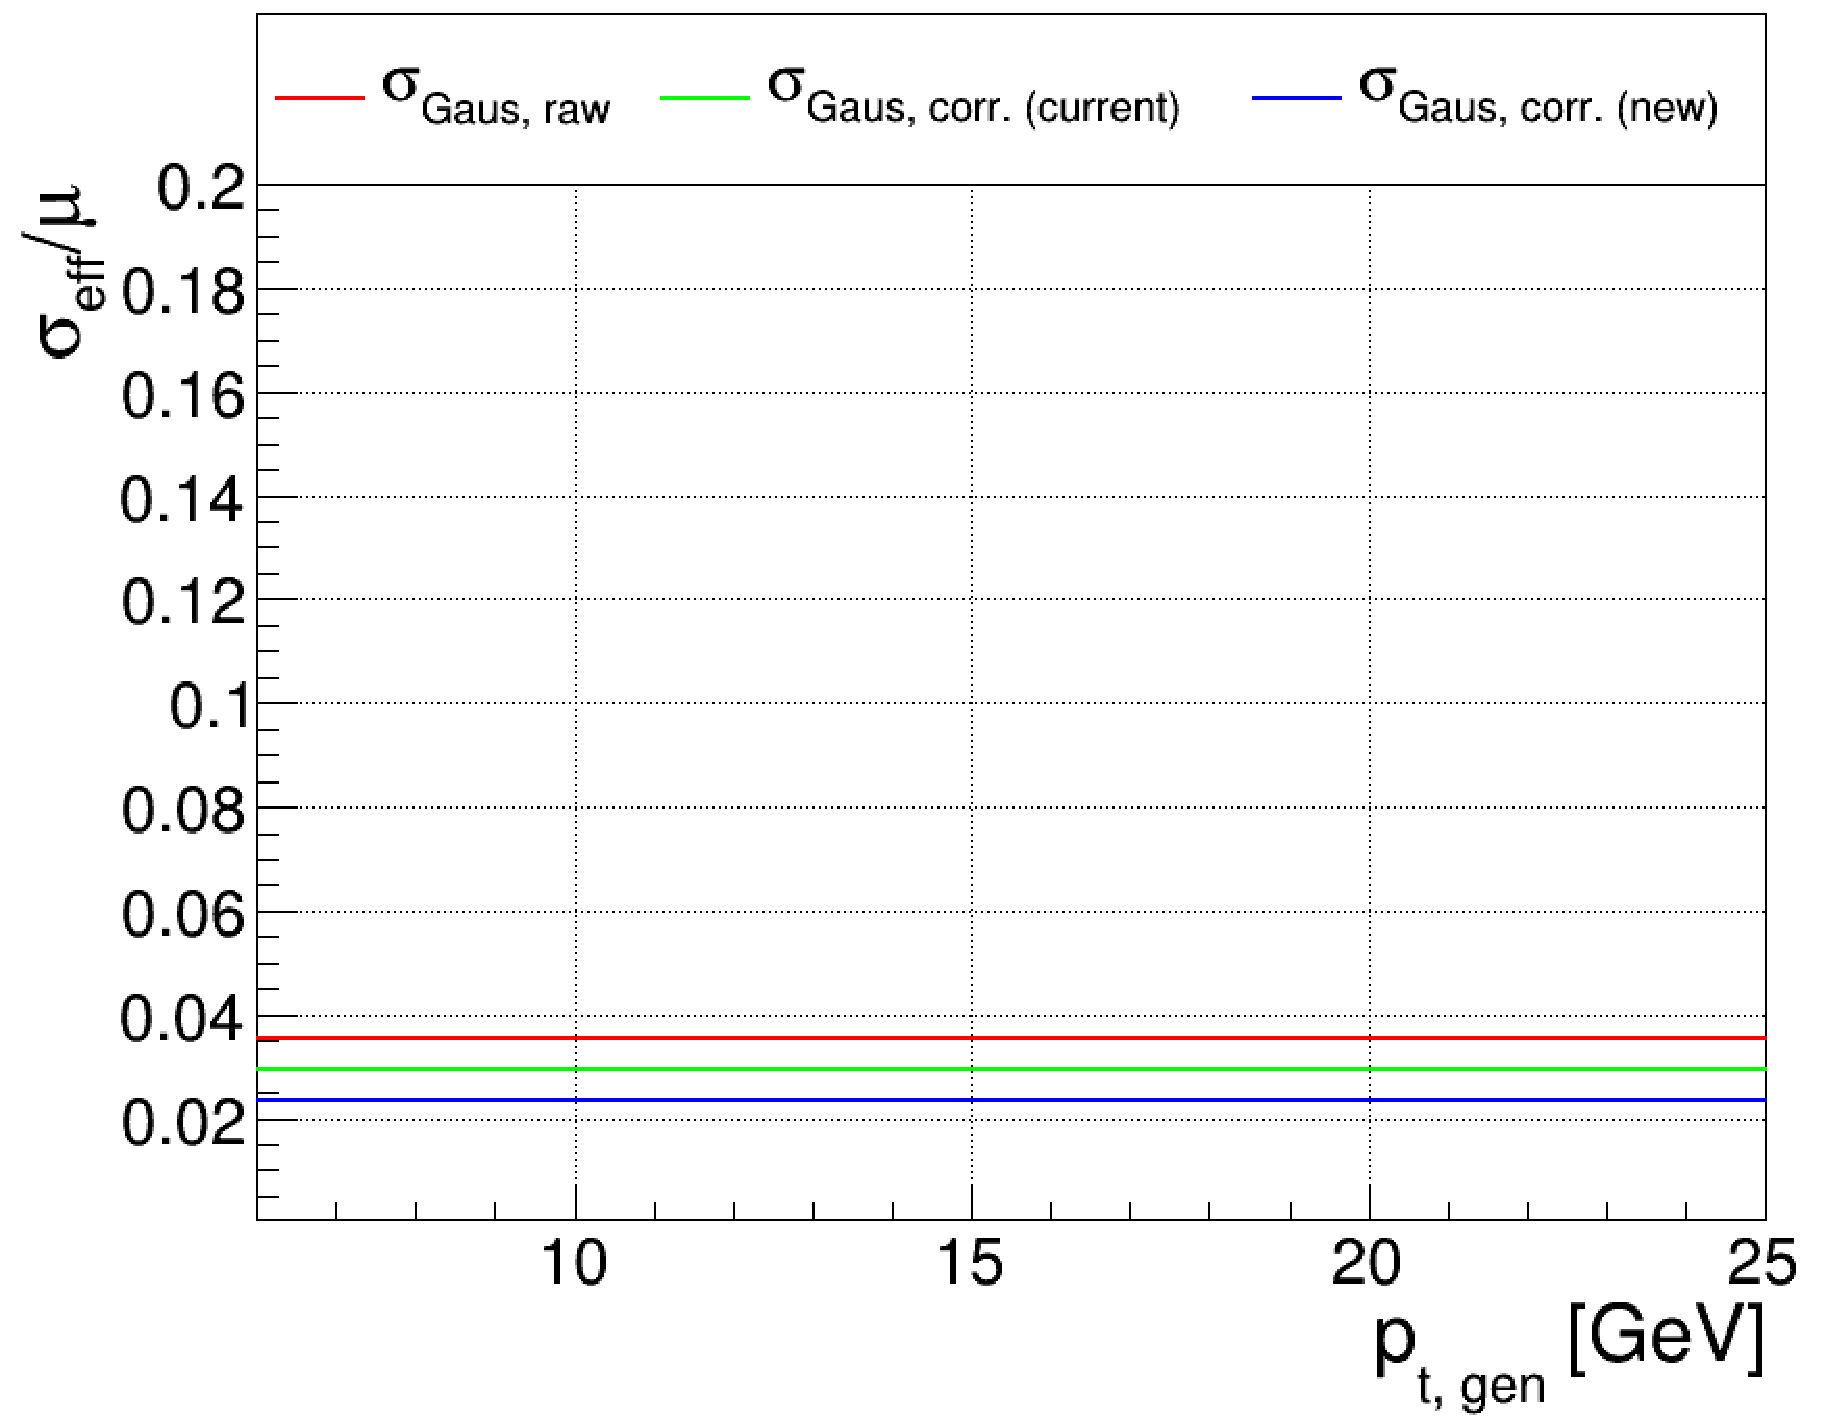
\includegraphics[width=0.495\textwidth]{./plots_pdf/ECAL_plots/plotsNOPU/EB/ZS/pdf/GENPT/EBZS_GENPT_0006_0025_EffSigmaOverBins.pdf}

%% 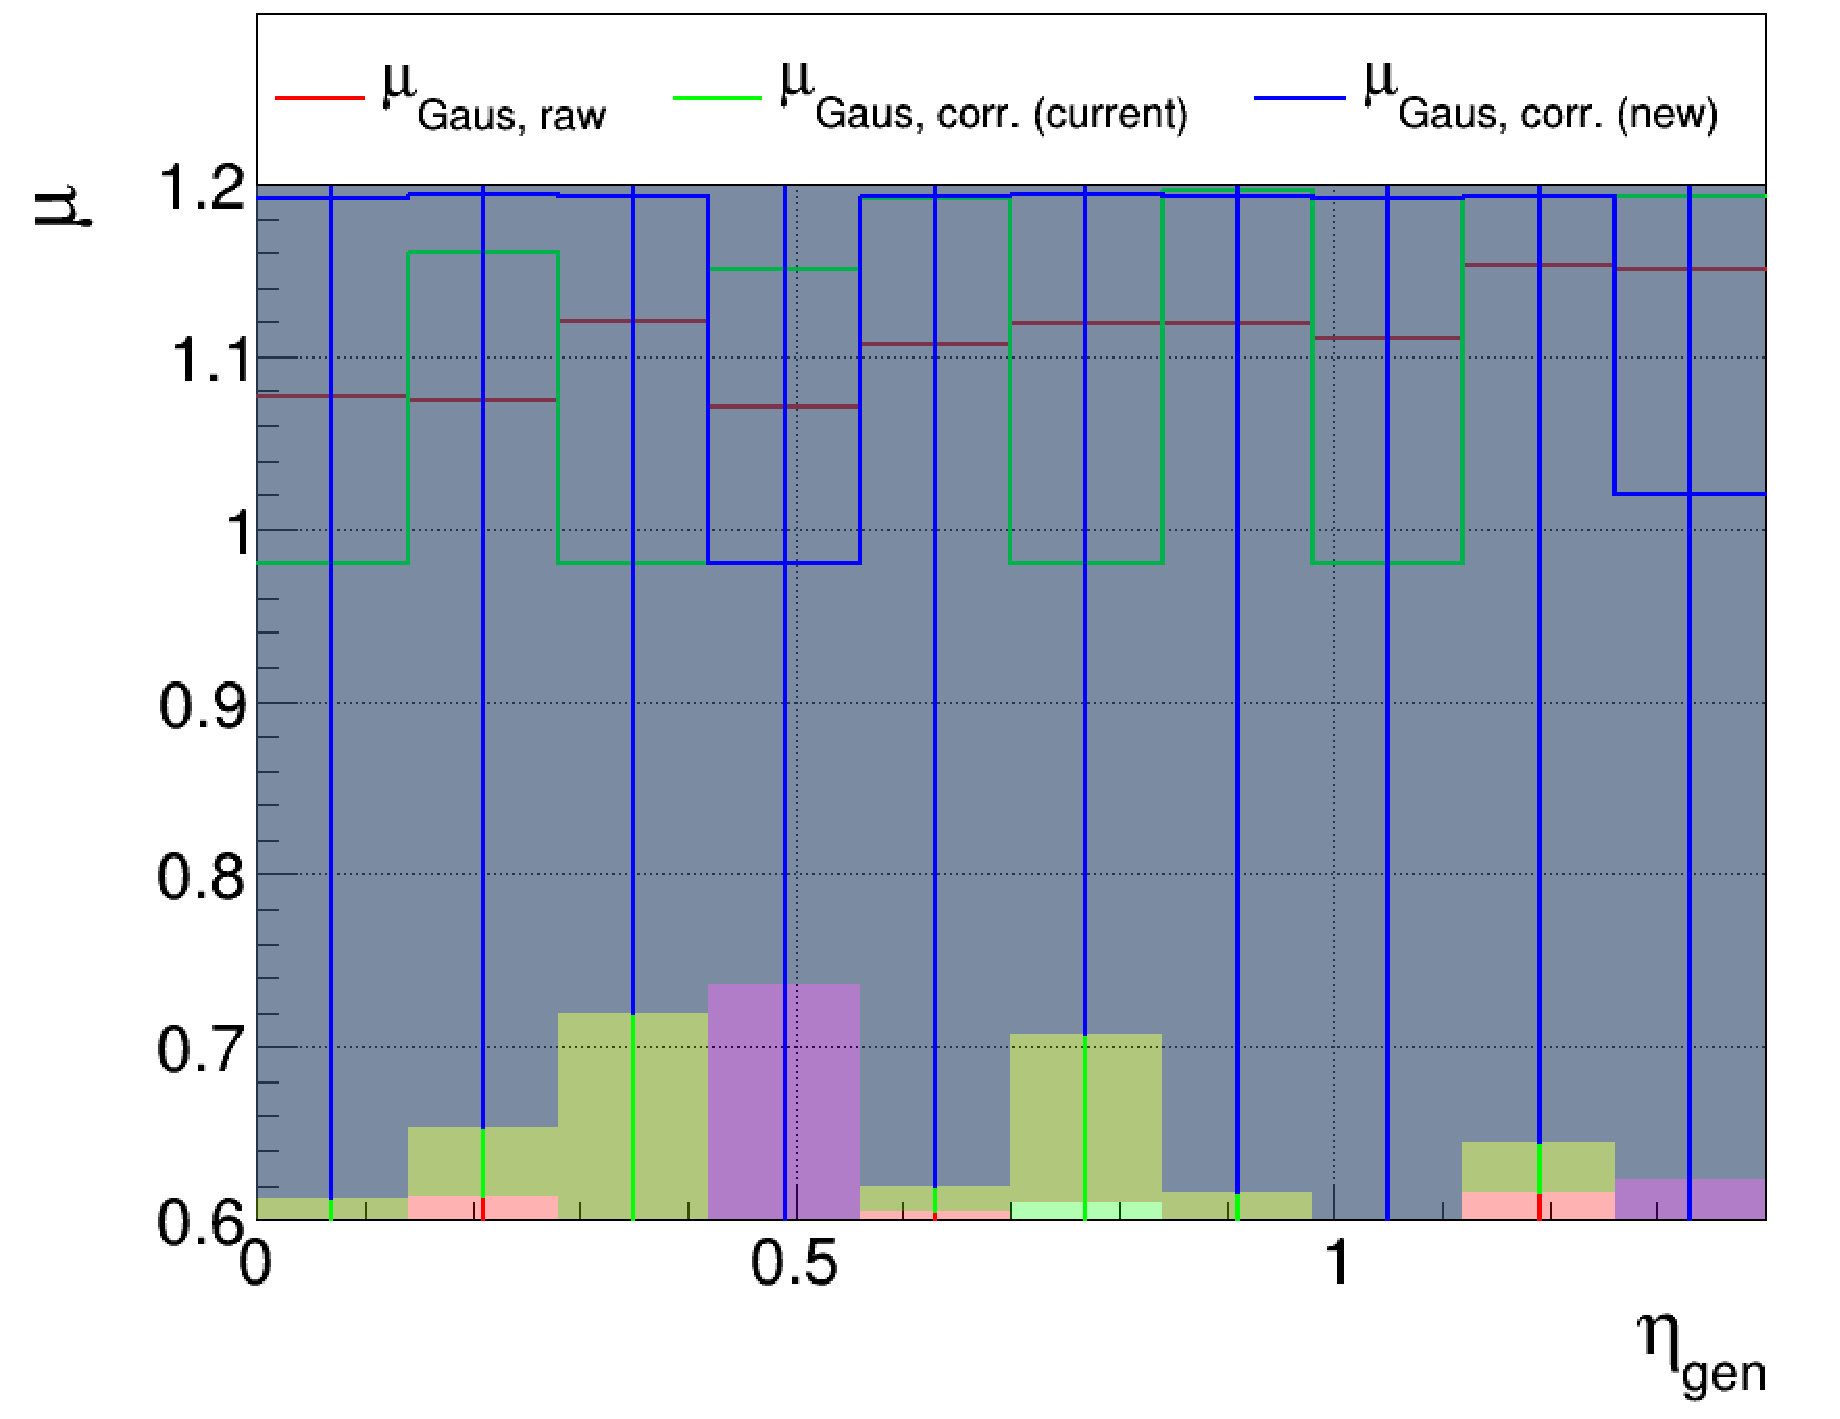
\includegraphics[width=0.495\textwidth]{./plots_pdf/ECAL_plots/plotsNOPU/EB/ZS/pdf/GENETA/EBZS_GENETA_0006_0025_MuOverBins.pdf}
%% 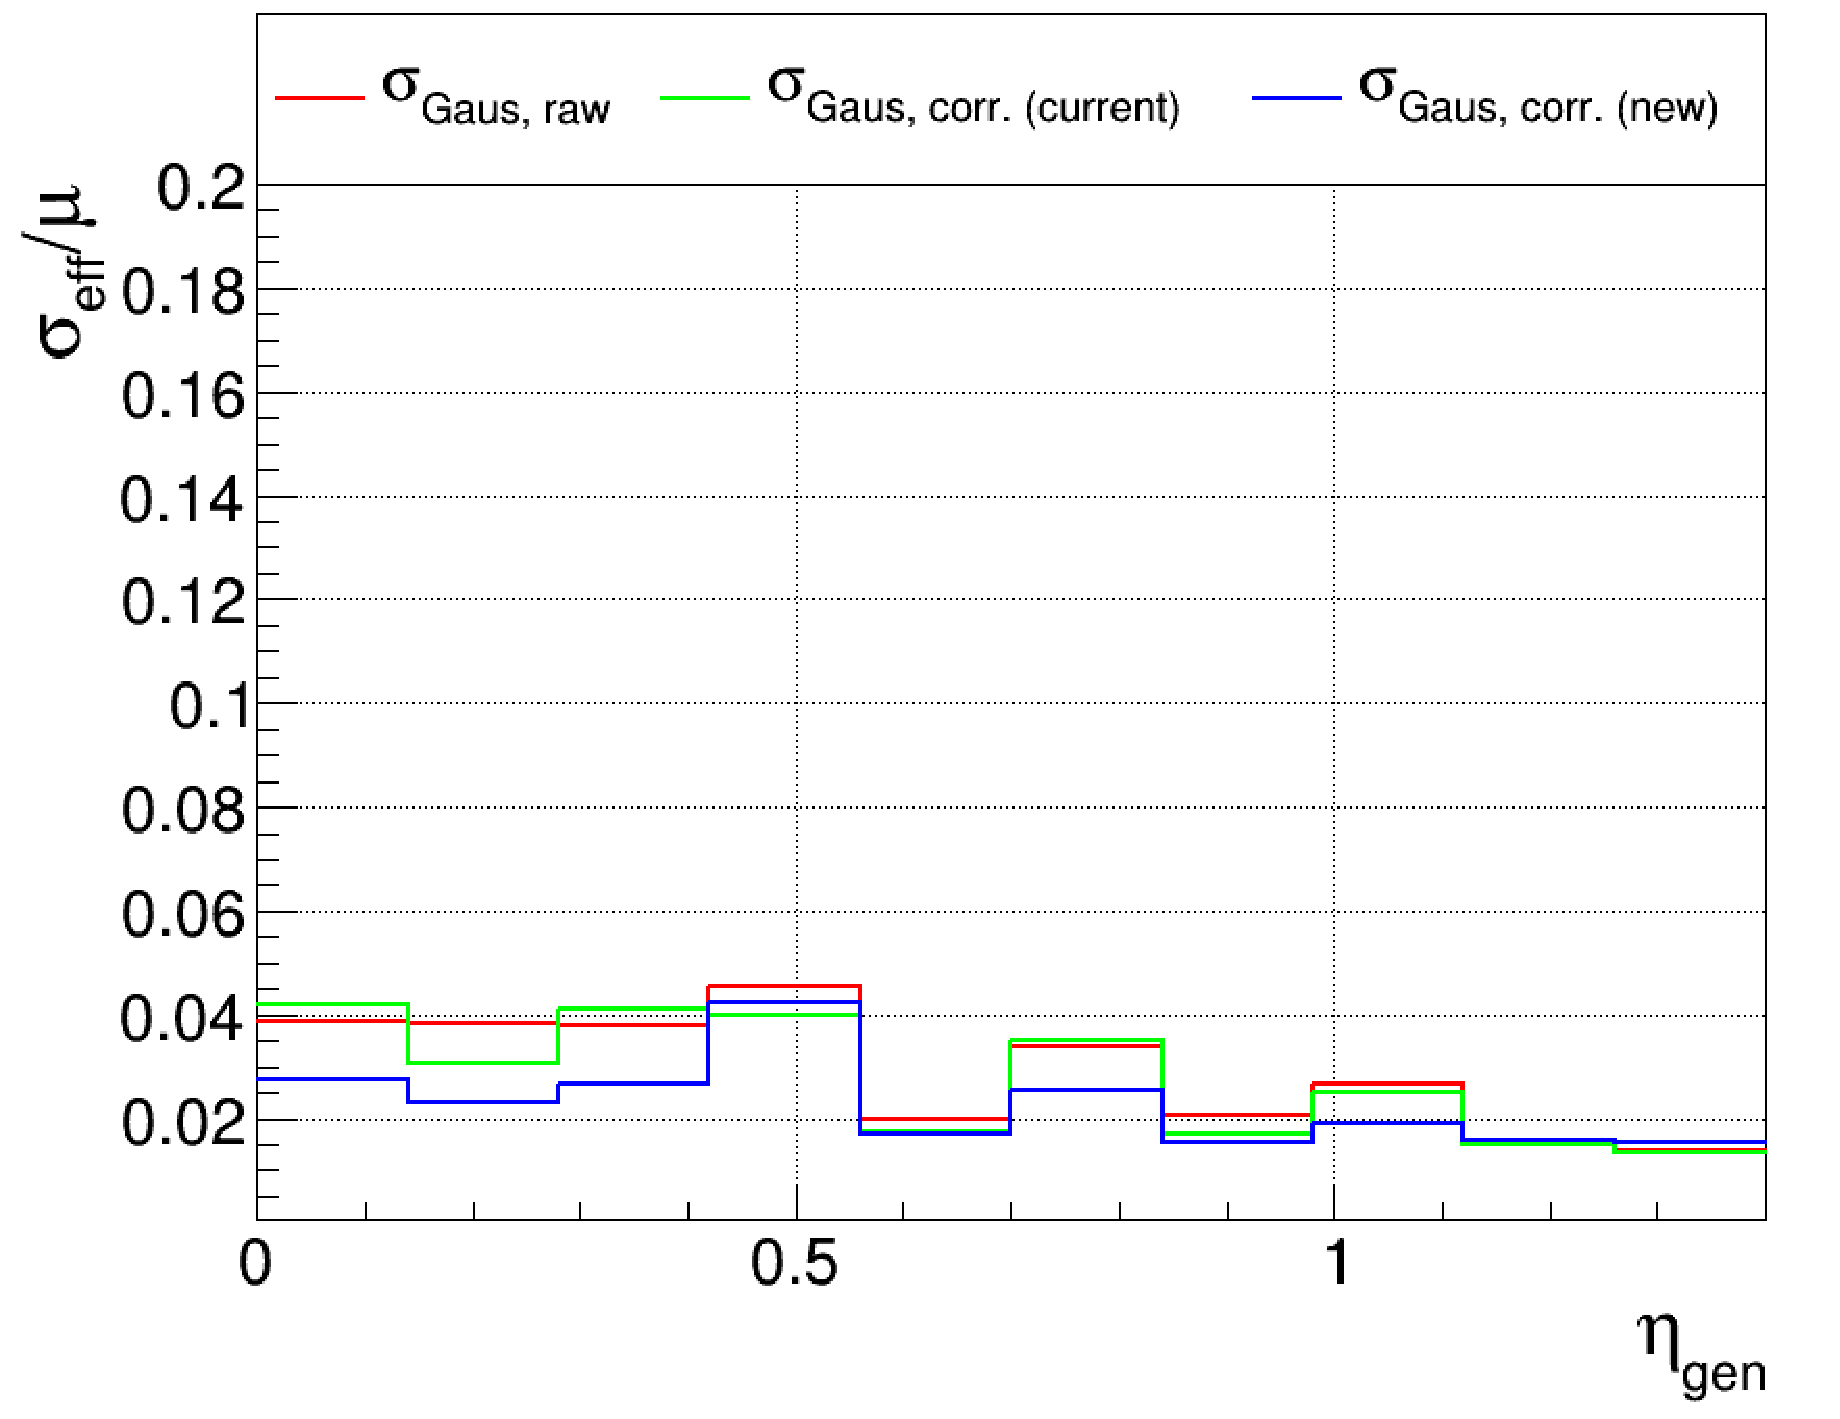
\includegraphics[width=0.495\textwidth]{./plots_pdf/ECAL_plots/plotsNOPU/EB/ZS/pdf/GENETA/EBZS_GENETA_0006_0025_EffSigmaOverBins.pdf}
%% \caption[]{EB - ZS Readout \pt 6-25\GeV}
%% \end{figure}




